% 图 27.3 —— 由 `checks/emit_hand.py` 自动拼出（probe 精测 + prims2 图元分解）
%%
% ⚠ 这是**稿子不是成品**：跑 `checks/checkhand.py 27.3` 看指标 + 看叠合图。
%%
%% ⚠ 待核：
%   · 本图 probe 报出阴影族 2 个 —— **本脚本不生成阴影**（要照原书手写）；prims2 的 strokes 里可能含阴影线，核对时留意别画重
%   · 可疑字形 2 项（空心圈 ⊙ 常被认成字母 o）—— 见文件末
%%
\documentclass[12pt]{standalone}
\usepackage{fontspec}
\setsansfont{Arial}
\newfontfamily\mfallback{DejaVu Sans}
\usepackage{tikz}
\begin{document}
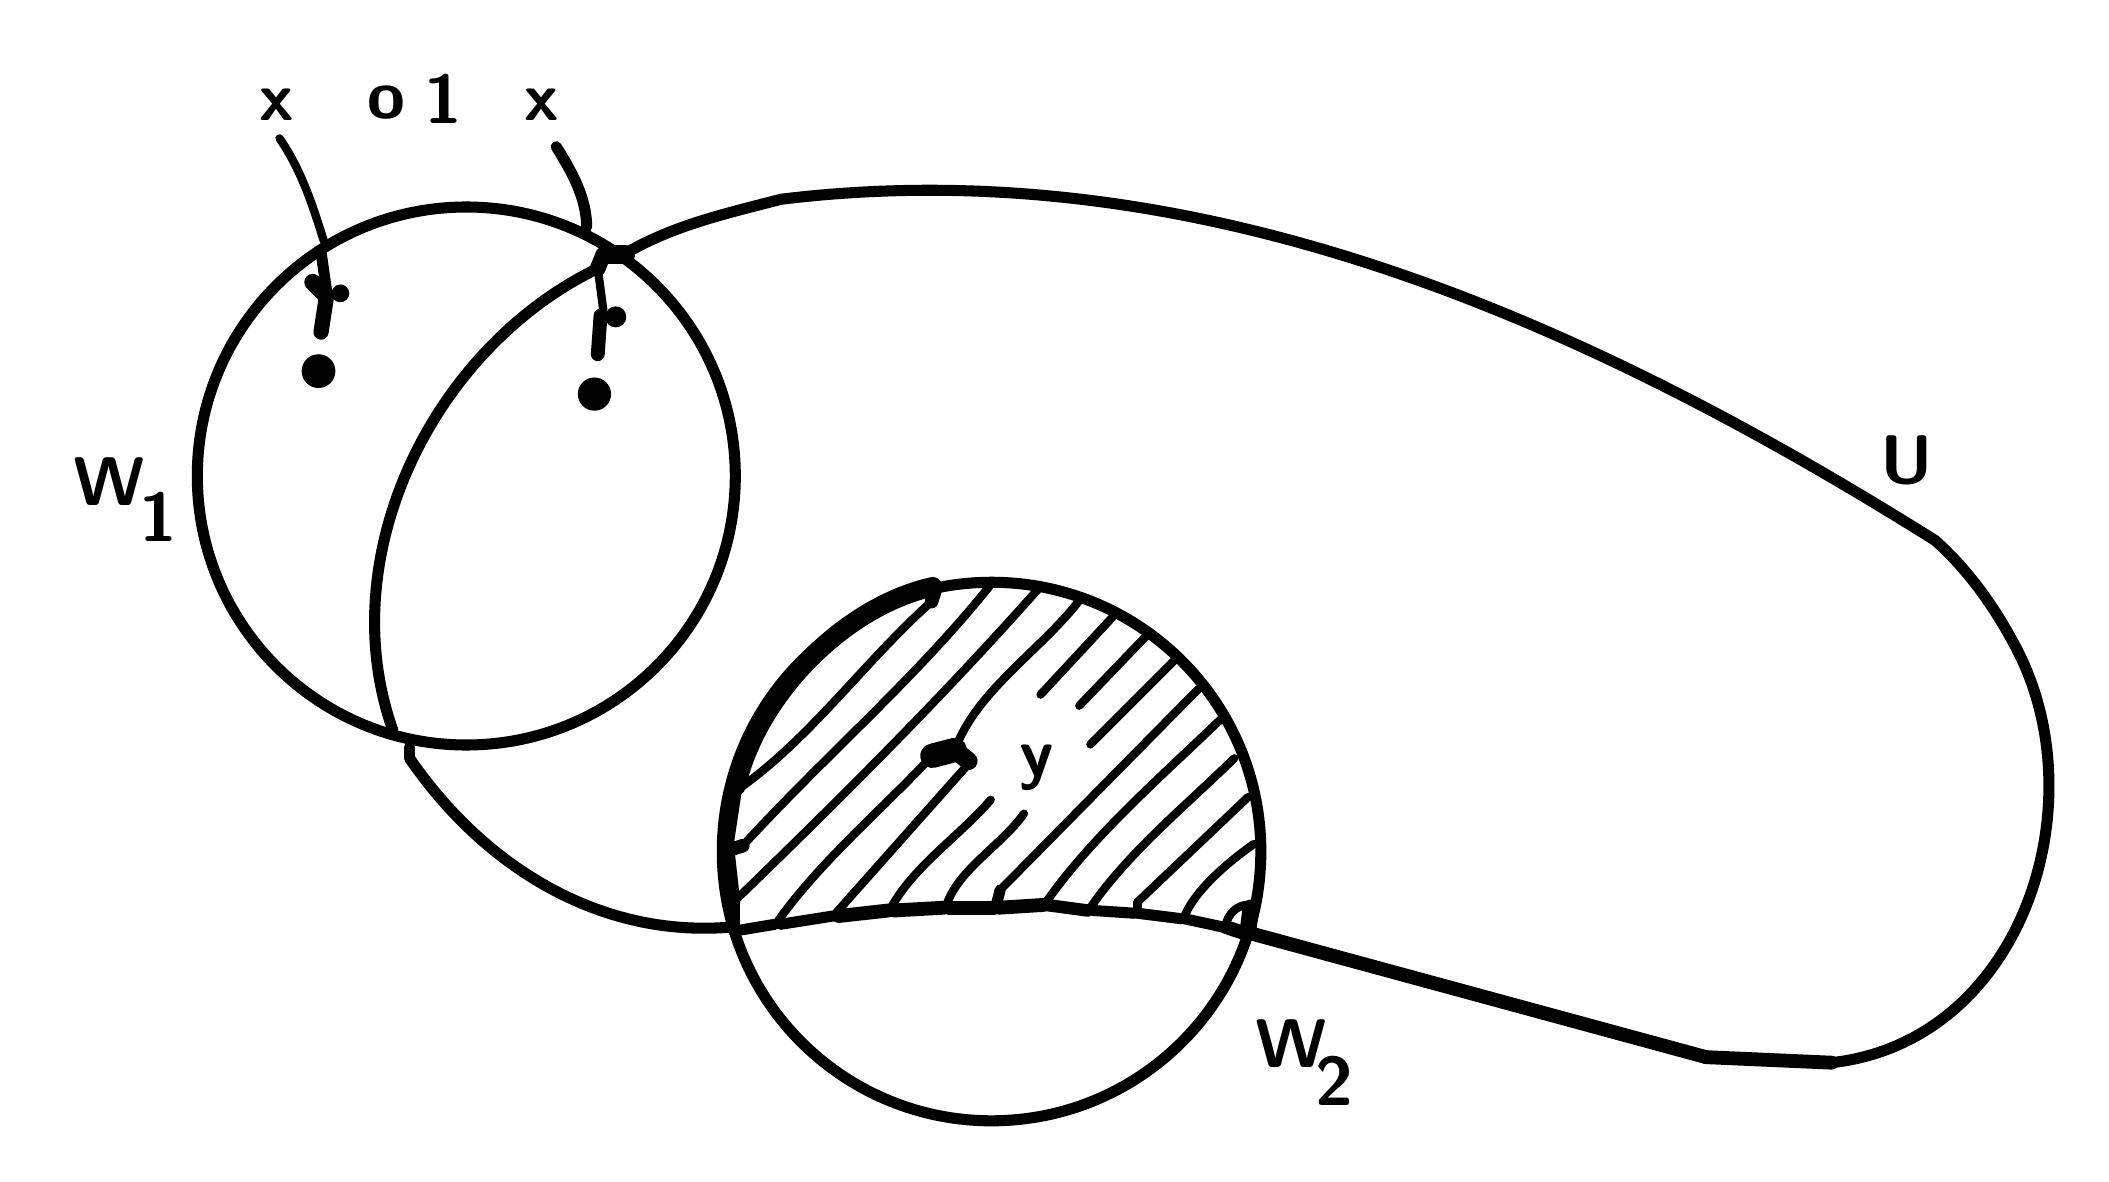
\begin{tikzpicture}[x=1pt, y=-1pt, line width=4.0pt, line cap=round, line join=round]

  %% ════ 填充区（prims2 的 fills）════

  %% ════ 直线段（prims2 的 strokes）════
  \draw[line width=4.0pt] (350.0,317.0) -- (351.4,311.6);
  \draw[line width=3.0pt] (351.4,311.6) -- (423.0,239.0);
  \draw[line width=4.9pt] (328.0,203.0) -- (326.6,207.4);
  \draw[line width=5.0pt] (333.0,318.0) -- (349.0,318.0);
  \draw[line width=3.0pt] (208.0,102.0) -- (206.0,87.0);
  \draw[line width=3.0pt] (384.0,259.0) -- (414.0,229.0);
  \draw[line width=5.0pt] (313.0,319.0) -- (331.0,318.0);
  \draw[line width=4.0pt] (256.0,276.0) -- (253.0,296.0);
  \draw[line width=4.0pt] (432.0,325.0) -- (418.0,322.0);
  \draw[line width=5.0pt] (255.0,316.0) -- (253.0,298.0);
  \draw[line width=5.0pt] (255.0,316.0) -- (255.0,324.0);
  \draw[line width=5.0pt] (651.9,374.0) -- (606.5,372.0);
  \draw[line width=5.0pt] (606.5,372.0) -- (441.0,327.0);
  \draw[line width=7.0pt] (216.0,82.0) -- (209.0,82.0);
  \draw[line width=3.0pt] (380.0,245.0) -- (404.0,220.0);
  \draw[line width=4.0pt] (417.0,322.0) -- (401.0,320.0);
  \draw[line width=8.8pt] (326.9,263.1) -- (335.0,261.0);
  \draw[line width=4.0pt] (270.0,324.0) -- (258.0,326.0);
  \draw[line width=4.5pt] (368.0,317.0) -- (383.0,319.0);
  \draw[line width=5.5pt] (108.0,97.0) -- (106.0,110.0);
  \draw[line width=6.1pt] (103.0,92.0) -- (107.0,96.0);
  \draw[line width=5.0pt] (351.0,318.0) -- (367.0,317.0);
  \draw[line width=6.5pt] (335.0,261.0) -- (340.0,265.0);
  \draw[line width=3.0pt] (366.0,241.0) -- (392.0,213.0);
  \draw[line width=6.0pt] (442.0,318.0) -- (441.0,326.0);
  \draw[line width=4.0pt] (272.0,324.0) -- (291.0,321.0);
  \draw[line width=4.0pt] (385.0,319.0) -- (400.0,320.0);
  \draw[line width=5.0pt] (206.0,118.0) -- (207.0,104.0);
  \draw[line width=5.0pt] (433.0,325.0) -- (439.0,327.0);
  \draw[line width=4.0pt] (108.0,95.0) -- (106.0,81.0);
  \draw[line width=5.7pt] (208.0,82.0) -- (206.0,87.0);
  \draw[line width=3.0pt] (401.0,319.0) -- (401.0,316.0);
  \draw[line width=3.0pt] (401.0,316.0) -- (441.0,278.0);
  \draw[line width=3.0pt] (340.0,266.0) -- (292.0,320.0);
  \draw[line width=4.9pt] (258.4,295.6) -- (254.0,297.0);
  \draw[line width=4.0pt] (138.0,260.0) -- (138.0,264.0);
  \draw[line width=5.0pt] (293.0,321.0) -- (311.0,319.0);

  %% ════ 曲线（prims2 的 curves —— 三段式，坐标同为 (y,x)）════
  \draw[line width=3.0pt] (326.6,207.4) .. controls (302.5,228.9) and (282.8,256.9) .. (257.0,275.0);
  \draw[line width=3.0pt] (255.0,316.0) .. controls (292.7,279.6) and (330.9,241.5) .. (365.0,203.0);
  \draw[line width=4.0pt] (217.0,81.0) .. controls (234.0,71.2) and (253.4,66.9) .. (272.2,62.0);
  \draw[line width=4.0pt] (272.2,62.0) .. controls (424.8,43.4) and (564.9,107.3) .. (689.3,185.3);
  \draw[line width=4.0pt] (689.3,185.3) .. controls (702.0,196.7) and (711.4,210.4) .. (719.0,225.0);
  \draw[line width=4.0pt] (719.0,225.0) .. controls (747.9,281.4) and (720.4,366.3) .. (651.9,374.0);
  \draw[line width=3.0pt] (360.0,284.0) .. controls (351.8,295.6) and (336.6,303.8) .. (332.0,317.0);
  \draw[line width=3.0pt] (91.0,40.0) .. controls (98.9,51.4) and (103.0,64.3) .. (107.0,77.0);
  \draw[line width=3.0pt] (418.0,321.0) .. controls (422.4,311.0) and (434.0,301.4) .. (443.0,295.0);
  \draw[line width=3.0pt] (312.0,318.0) .. controls (320.1,303.1) and (336.5,292.3) .. (348.0,279.0);
  \draw[line width=3.0pt] (271.0,323.0) .. controls (286.2,301.5) and (308.2,283.0) .. (326.9,263.1);
  \draw[line width=3.0pt] (380.0,207.0) .. controls (366.2,224.9) and (342.9,239.5) .. (335.0,261.0);
  \draw[line width=3.0pt] (441.0,317.0) .. controls (437.2,316.8) and (433.6,320.5) .. (433.0,324.0);
  \draw[line width=4.0pt] (202.0,72.0) .. controls (201.9,61.2) and (196.5,51.9) .. (191.0,43.0);
  \draw[line width=3.0pt] (436.0,264.0) .. controls (418.5,281.1) and (397.5,298.3) .. (384.0,318.0);
  \draw[line width=3.0pt] (349.0,200.0) .. controls (322.2,234.0) and (288.1,263.1) .. (258.4,295.6);
  \draw[line width=4.0pt] (132.0,254.0) .. controls (109.4,190.4) and (147.0,115.5) .. (206.0,87.0);
  \draw[line width=4.0pt] (138.0,264.0) .. controls (164.7,302.9) and (206.4,329.0) .. (254.0,325.0);
  \draw[line width=7.0pt] (256.0,274.0) .. controls (263.4,241.5) and (294.6,209.3) .. (327.0,202.0);
  \draw[line width=3.0pt] (368.0,316.0) .. controls (384.4,292.5) and (409.4,270.8) .. (431.0,250.0);

  %% ════ 圆 / 椭圆（probe 精测）════
  \draw (158.5,162.0) circle (97.2);
  \draw (348.3,297.7) circle (97.3);

  %% ════ 实心点 ════
  \fill (105.1,124.1) circle (6.1);
  \fill (204.8,132.4) circle (6.0);
  \fill (113.0,96.0) circle (3.2);
  \fill (212.5,104.5) circle (3.8);

  %% ════ 标签（probe 直接给的 \node 行）════
  %% ⚠ 全部补了 fill=white：文字在最上层，否则与曲线交叉干扰
     \node[anchor=center,inner sep=0pt,fill=white,font=\fontsize{30.5}{38.1}\selectfont] at (129.8,27.0) {\textsf{\textbf{\textit{o}}}};   % box(121,17,16,17)
     \node[anchor=center,inner sep=0pt,fill=white,font=\fontsize{27.4}{34.2}\selectfont] at (150.2,26.0) {\textsf{\textbf{1}}};   % box(142,17,10,17)
     \node[anchor=center,inner sep=0pt,fill=white,font=\fontsize{28.3}{35.4}\selectfont] at (89.9,27.9) {\textsf{\textbf{\textit{x}}}};   % box(81,18,16,16)
     \node[anchor=center,inner sep=0pt,fill=white,font=\fontsize{28.3}{35.4}\selectfont] at (185.9,27.9) {\textsf{\textbf{\textit{x}}}};   % box(177,18,16,16)
     \node[anchor=center,inner sep=0pt,fill=white,font=\fontsize{29.6}{37.0}\selectfont] at (679.0,156.2) {\textsf{\textbf{\textit{U}}}};   % box(669,144,20,22)
     \node[anchor=center,inner sep=0pt,fill=white,font=\fontsize{28.7}{35.8}\selectfont] at (29.7,164.0) {\textsf{\textbf{\textit{W}}}};   % box(17,152,25,22)
     \node[anchor=center,inner sep=0pt,fill=white,font=\fontsize{22.9}{28.6}\selectfont] at (47.2,176.9) {\textsf{\textbf{1}}};   % box(41,168,7,17)
     \node[anchor=center,inner sep=0pt,fill=white,font=\fontsize{29.8}{37.3}\selectfont] at (364.7,267.2) {\textsf{\textbf{\textit{y}}}};   % box(356,254,17,23)
     \node[anchor=center,inner sep=0pt,fill=white,font=\fontsize{28.7}{35.8}\selectfont] at (456.7,367.0) {\textsf{\textbf{\textit{W}}}};   % box(444,355,25,22)
     \node[anchor=center,inner sep=0pt,fill=white,font=\fontsize{23.6}{29.6}\selectfont] at (472.1,380.9) {\textsf{\textbf{2}}};   % box(466,372,11,17)

  % 钉死画布：否则超出的图元/控制点会把页面撑大，1:1 回比就失准
  \pgfresetboundingbox
  \path[use as bounding box] (0,0) rectangle (742,407);
\end{tikzpicture}
\end{document}

% ⚠ 待核清单（probe 拿不准，人眼过一遍）：
%   · 可疑字形：\node[anchor=center,inner sep=0pt,font=\fontsize{30.5}{38.1}\selectfont] at (129.8,27.0) {\textsf{\textbf{\tex
%   · 未识别/跳过：⑤ 跳过/未识别的字形
